\section{High level system overview}
This section addresses high level system design especially.
\begin{itemize}
    \item data structure and data flow
    \item sequential interaction between the system subcomponents
\end{itemize}

\subsection{Data structure and data flow}
We assume that the IMU will provide the following data:
\begin{itemize}
    \item $a_x$ acceleration on the x-axis
    \item $a_y$ acceleration on the y-axis
    \item $a_z$ acceleration on the z -axis
    \item $\omega_x$ angular rate along its x-axis
    \item $\omega_y$ angular rate along its y-axis
    \item $\omega_z$ angular rate along its z-axis
    \item $T$ temperature of the sensor.
\end{itemize}
We assume that the physical sampling of all those values are made at the exact same time, respectively the difference between the sampling time is negligible.
In other word we can timestamp the measurment time with a single timestamp $t_mes$.

\subsection{Sequential interaction}

\begin{figure}[ht]
    \centering
    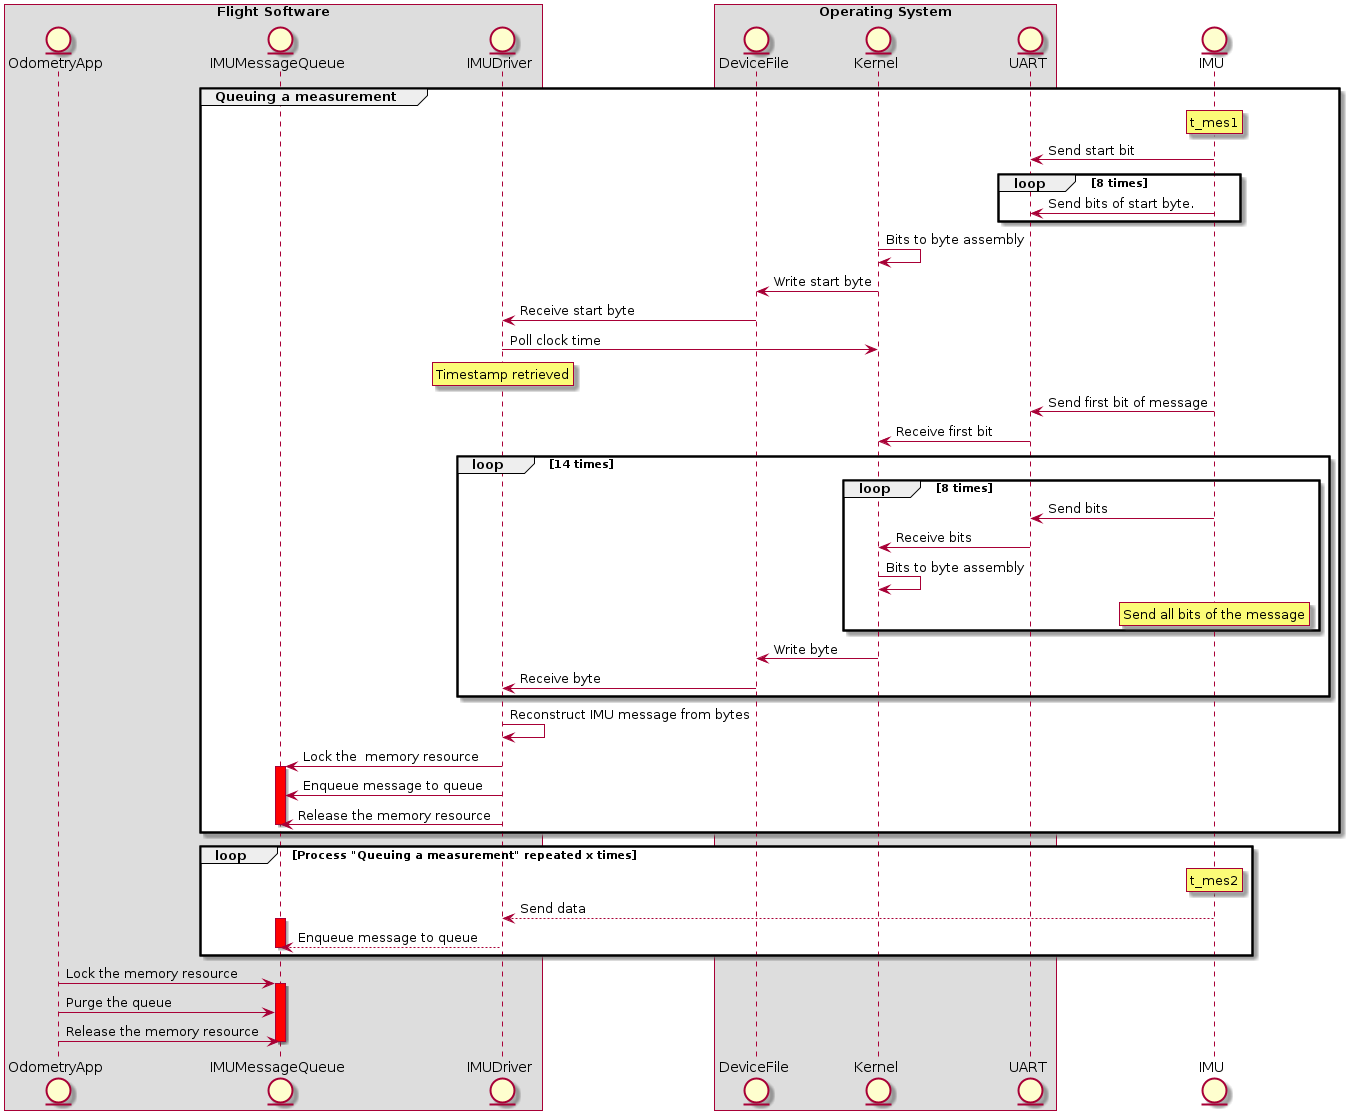
\includegraphics[width=1.0 \textwidth]{diagrams/high_level_sys_overview.png}
    \caption{High level sequence diagram of the nominal operation case}
    \label{reference}
\end{figure}

\subsection{Fault-tree analysis}

\subsection{Interface definition}
